\documentclass[compress, 8pt]{beamer}
% \documentclass[handout, 8pt]{beamer}
\usepackage[utf8]{inputenc}

% Notes to self: \nts[color option]{text that is a note}
\newif\ifshowcomments
% \showcommentstrue % uncomment to show
\input{preambleB}

%%%%%%%%%%%%%%%%%%%%%%%%%%%%%%%%%%%%%%%%%%%%%%%%%%%%%%%%%%%%%%%%%%%%%%%%%%%%%%
% Paths to figures
\usepackage{subcaption}

% Avoid a warning on mac; can introduce a warning (and maybe a break) on windows
% \usepackage{etex}
% Avoid a warning
\let\Tiny=\tiny

%Information to be included in the title page:
\title{Probability Review}
\subtitle{ECON726}
\author[]{Tara Sullivan}
\institute{
Tara Sullivan \\
\textit{tara.sullivan55@login.cuny.edu}
}
\date{
\today
\nts{\\
\medskip
Notes/comments are in gray and will be excluded from the presentation.
}
}

% plot graphs with pgfplots
\usepackage{pgfplots}
\pgfplotsset{compat=newest}
\usepgfplotslibrary{groupplots}
\usepgfplotslibrary{dateplot}
\pgfplotsset{compat=newest,
    every axis/.style={
        axis y line*=left,
        axis x line*=bottom,
        % allows for multi-line legend entries
        legend style={cells={align=left}},
        % allows for multi-line titles
        title style={align=center},
    },
}

% For animations using underbrace 
% Source: https://tex.stackexchange.com/a/565866
\usepackage{xparse, letltxmacro}
\LetLtxMacro{\oldunderbrace}{\underbrace}
\DeclareDocumentCommand{\underbrace}{d<> m e{_}}{%
  \IfValueTF{#1}{% IF <overlay-specification> given
    % using global onlside flag, cf. p82 beamer manual v3.59
    \oldunderbrace{#2\onslide<#1>}_{#3}\onslide%
  }{% ELSE
    \oldunderbrace{#2}_{#3}
  }%
}%

%%%%%%%%%%%%%%%%%%%%%%%%%%%%%%%%%%%%%%%%%%%%%%%%%%%%%%%%%%%%%%%%%%%%%%%%%%%%%%%%
\begin{document}    
%\beamertemplatenavigationsymbolsempty


%%%%%%%%%%%%%%%%%%%%%%%%%%%%%%%%%%%%%%%%%%%%%%%%%%%%%%%%%%%%%%%%%%%%%%%%%%%%%%%%
\begin{frame}
\titlepage
% \tikzset{external/figure name={intro_}}
\end{frame}

\begin{frame}{Housekeeping}

Homework 1:
\begin{itemize}
    \item Important: \textbf{Include the link to GitHub; this will be penalized in the future} 
    \item Please submit if you have not! Otherwise you will get a zero (this worked out to 2.5 points on your final grade last year!)
\end{itemize}

\vspace{3ex}
Python instruction:
\begin{itemize}
    \item Next week, we'll do some python introduction alongside statistical review
    \item Please bring your computer if you'd like to follow along.
\end{itemize}

\vspace{3ex}
Homework this week:
\begin{itemize}
    \item Homework this week: submit 1-2 possible papers for your project. Be ambitious and creative!
    \item Read \emph{Mostly Harmless} Chapter 1 \& 2
    \item Due in 2 weeks: Probability review questions. please submit a \textbf{handwritten} response.
\end{itemize}

\vspace{3ex}
Agenda:
\begin{itemize}
    \item Discuss resource for looking for papers %: \url{https://www.aeaweb.org/journals}
    \item Probability review
\end{itemize}

\end{frame}

%%%%%%%%%%%%%%%%%%%%%%%%%%%%%%%%%%%%%%%%%%%%%%%%%%%%%%%%%%%%%%%%%%%%%%%%%%%%%%%


%%%%%%%%%%%%%%%%%%%%%%%%%%%%%%%%%%%%%%%%%%%%%%%%%%%%%%%%%%%%%%%%%%%%%%%%%%%%%%%%
\begin{frame}{Paper}

Recall our goal: replicate and extend a paper using the methods from this class.

\vspace{3ex}
Methods we'll definitely cover in this class:
\begin{itemize}
    \item Causal linear regression (under unconfoundedness/with selection on observables/under conditional independence assumption)
    \item Matching (especially propensity score matching)
    \item Panel data methods (especially differences-in-differences; synthetic control)
\end{itemize}

\vspace{3ex}
Other methods we may cover:
\begin{itemize}
    \item Instrumental variables
    \item Additional panel data methods (i.e. fixed and random effects models/unobserved effects models)
    \item Regression discontinuity designs (sharp RD, fuzzy RD)
    \item Machine learning methods (lasso, random forest)
\end{itemize}


\end{frame}

%%%%%%%%%%%%%%%%%%%%%%%%%%%%%%%%%%%%%%%%%%%%%%%%%%%%%%%%%%%%%%%%%%%%%%%%%%%%%%%%
\begin{frame}{This week's assignment}

Think of causal questions you would like to answer in this class:

\begin{itemize}
    \item This is your opportunity to be a bit more ambitious 

    \vspace{1ex}
    \item You will not be locked in to this topic choice; you can always fall back on an easier paper topic later

    \vspace{1ex}
    \item Remember your goal is to \textbf{replicate} and \textbf{extend} this project 
    \begin{itemize}
        \item If you pick a more difficult paper, you can focus on the replication. 
        \item If you pick an easier paper, you can focus on the extension
    \end{itemize}

    \vspace{1ex}
    \item YOUR GOAL IS TO AVOID CLEANING DATA (specifically for the replication part of the assignment). This is far and away the most time intensive part of beginning a project
    \begin{itemize}
        \item When you submit your final code, \textbf{I} will not run any code that cleans data
    \end{itemize}

    \vspace{1ex}
    \item You want PUBLISHED papers whose data/replication package is posted online
    \begin{itemize}
        \item Not NBER working papers
        \item Not American Economic Review: Papers \& Proceedings
    \end{itemize}
\end{itemize}

\end{frame}

%%%%%%%%%%%%%%%%%%%%%%%%%%%%%%%%%%%%%%%%%%%%%%%%%%%%%%%%%%%%%%%%%%%%%%%%%%%%%%%%
\begin{frame}
Good resource for finding papers (we'll discuss next class): \url{https://paulgp.com/econlit-pipeline/index.html}
\begin{itemize}
    \item Look up a methodology ``difference-in-differences''
    \item Search for a paper with replication data

    \item Don't limit yourself to this website; it was made with AI and might not capture everything!
\end{itemize}

\vspace{2ex}
Partial vs full replication data:
\begin{itemize}
    \item This likely has not been validated by a person, so proceed with caution, and validate yourself
    \item For this assignment, you need to replicate \textbf{key results}
    \item It's okay if data are partially available if it means you can replicate key results!
\end{itemize}
\end{frame}

%%%%%%%%%%%%%%%%%%%%%%%%%%%%%%%%%%%%%%%%%%%%%%%%%%%%%%%%%%%%%%%%%%%%%%%%%%%%%%%%
\begin{frame}{Checking data is accessible}
Suppose you are considering this paper: \url{https://doi-org.proxy.wexler.hunter.cuny.edu/10.1093/qje/qjab004}
\begin{itemize}
    \item Very cool and relevant paper
    \item Data and replication code available on the paper website
\end{itemize}
\begin{quote}
    Code replicating the figures and tables in this article can be found in Miller, Johnson, and Wherry (2021), in the Harvard Dataverse doi: 10.7910/DVN/UEJRKH.
\end{quote}
Go to the doi website: \url{https://doi.org/10.7910/DVN/UEJRKH}
\begin{itemize}
\item Before doing anything else, find the README
\end{itemize}

\begin{quote}
    Restricted-use Census data: The main analysis of this paper relies on the 2008-2013 waves of the American Community Survey linked to the 2018 Q2 Numident File and the 2008-2016 MSIS and TMSIS files from CMS documenting Medicaid enrollment. Refer to Appendix Section 1 for additional information on the years covered by MSIS and TMSIS versions of this file. 

    \vspace{2ex}
Researchers may obtain access to these data through the Census Federal Statistical Research Data Center (FSRDC) system. Researchers can learn more about how to access restricted use data through the Census FSRDC here: https://www.census.gov/about/adrm/fsrdc.html.
\end{quote}

$\implies$ \textbf{Sometimes you need to dig deep to figure out if the paper is replicable}

\end{frame}

%%%%%%%%%%%%%%%%%%%%%%%%%%%%%%%%%%%%%%%%%%%%%%%%%%%%%%%%%%%%%%%%%%%%%%%%%%%%%%%%
\begin{frame}{How to find a paper}

Note on papers
\begin{itemize}
    \item Think of topics you are interested in, like the impact of labor supply on wages
    \item Look through recent issues of top journals. See if anything catches your eye. In the past five or so years, these journals require replication packages: \url{https://www.aeaweb.org/journals}

    \item Try to find papers that use the methods we discuss in class.
\end{itemize}

\vspace{2ex}
Where to poke around and look for papers:
\begin{itemize}
    \item MHE data archives: you know this data is usable and clean!: \url{https://economics.mit.edu/people/faculty/josh-angrist/mhe-data-archive}
    \item Angrist, the author of MHE, also has many datasets available on his website for his papers: \url{https://economics.mit.edu/people/faculty/josh-angrist/angrist-data-archive}
    \item Maybe explore another famous professor's page: \url{https://davidcard.berkeley.edu/papers.html}
    \item Or look at their students’: \url{https://about.peterhull.net/publications}
    \item Look for ``code'', ``data'', ``replication package'' etc. That means the data is cleaned; this is huge!

\end{itemize}


\end{frame}

%%%%%%%%%%%%%%%%%%%%%%%%%%%%%%%%%%%%%%%%%%%%%%%%%%%%%%%%%%%%%%%%%%%%%%%%%%%%%%%%
\begin{frame}{Selecting a paper}

Top 5 economics journals:
\begin{itemize}
    \item American Economic Review
    \begin{itemize}
        \item Note: American Economic Review: Papers and Proceedings are short papers and are NOT sufficient for this assignment
    \end{itemize}
    \item Econometrica
    \item Journal of Political Economy
    \item Quarterly Journal of Economics
    \item Review of Economic Studies
\end{itemize}
Also good:
\begin{itemize}
    \item American Economic Journal: Applied Economics
    \item Journal of Public Economics
    \item Review of Economics and Statistics
\end{itemize}
% Here is a random list online of good [economics] journals: \url{https://www.stern.nyu.edu/sites/default/files/assets/documents/Econ%20Top%20Journals%20-%20July%202020.pdf}



\end{frame}

% %%%%%%%%%%%%%%%%%%%%%%%%%%%%%%%%%%%%%%%%%%%%%%%%%%%%%%%%%%%%%%%%%%%%%%%%%%%%%%%%
% \begin{frame}{Example of how this reasoning can go}

% Let's say you are interested in the impact of labor supply on wages:
% item
% \begin{itemize}
%     \item David Card wrote a famous paper in 1991: \url{https://davidcard.berkeley.edu/papers/mariel-impact.pdf} 
%     \item Looks promising, it's methodologically pretty simple!
%     \item Unfortunately there doesn't appear to be replication code
%     But some googling leads me to find a different paper that tests these methods using synthetic control, a method we'll cover in this class! \url{https://giovanniperi.ucdavis.edu/data-for-peri-and-yasenov.html}
%     \begin{itemize}
%         \item It seems this paper is published at the Journal of Human Resources, but the data online might be from a different version. That's also okay! 
%     \end{itemize}
% \end{itemize}

% \end{frame}

%%%%%%%%%%%%%%%%%%%%%%%%%%%%%%%%%%%%%%%%%%%%%%%%%%%%%%%%%%%%%%%%%%%%%%%%%%%%%%%%
\section[Introduction]{Probability and Causality}
\miniframesoff
\begin{frame}
    \tableofcontents[currentsection]
\end{frame}
\miniframeson

%%%%%%%%%%%%%%%%%%%%%%%%%%%%%%%%%%%%%%%%%%%%%%%%%%%%%%%%%%%%%%%%%%%%%%%%%%%%%%%%
\begin{frame}{Probability and Causality}

At first glance, it's strange that causality and probability are closely intertwined. 

\begin{itemize}
    \item Causality: cause and effect; law-like
    \item Probability: uncertainty
\end{itemize}

\pause
\vspace{2ex}
Causal reasoning is often used in situations that are rife with uncertainty
\begin{itemize}
    \item Drunk driving causes accidents
    \item If you don't study in college, you will fail
\end{itemize}

\pause
\vspace{2ex}
$\implies$ Causal theory must account for uncertainty

\end{frame}


%%%%%%%%%%%%%%%%%%%%%%%%%%%%%%%%%%%%%%%%%%%%%%%%%%%%%%%%%%%%%%%%%%%%%%%%%%%%%%%%
\begin{frame}{Probability and Causality (cont.)}

Many quantitative fields use probability theory as the backbone of their causal theory

\vspace{3ex}
Want to account for:
\begin{itemize}
    \item Presence of causal connections
    \item Relative strength of those connections
    \item Ways of inferring connections from noisy data
\end{itemize}

\vspace{3ex}
Probability theory allows us to tolerate unexplained exceptions in causal expressions
\begin{enumerate}
    \item My neighbors roof gets wet whenever mine does
    \item If I hose my roof then it will get wet
\end{enumerate}
Contradictory statements are allowed under probability theory

\end{frame}

%%%%%%%%%%%%%%%%%%%%%%%%%%%%%%%%%%%%%%%%%%%%%%%%%%%%%%%%%%%%%%%%%%%%%%%%%%%%%%%%
\begin{frame}{Understanding probability}

We'll do a fast review of probability!
\begin{itemize}
    \item First, we discuss the basic laws of probability in terms of events
    \begin{itemize}
        \item Axioms of probability and basic laws
        \item Independence
        \item Conditional probability
    \end{itemize}
    \item We then talk about random variables
    \begin{itemize}
        \item Informally, random variables are just a way of assigning a numerical value to a probabilistic event
        \item Probability distributions
        % \item Expected value and conditional expected value
    \end{itemize}
    \item When appropriate, I'll discuss the concept of directed acyclic graphs (DAGs)
    \begin{itemize}
        \item Fundamental to machine learning theory and causal theory!

    \end{itemize}

\end{itemize}

Easiest way to approach this:
\begin{itemize}
    \item Keep concrete examples in mind (rolling one die, rolling two dice)
    \item Focus on discrete, be confident things generalize to continuous
\end{itemize}


Great resource, if you like to read or want to learn more: \emph{Causality} by Judea Pearl (especially chapter 1)

\end{frame}
    
%%%%%%%%%%%%%%%%%%%%%%%%%%%%%%%%%%%%%%%%%%%%%%%%%%%%%%%%%%%%%%%%%%%%%%%%%%%%%%%%

%%%%%%%%%%%%%%%%%%%%%%%%%%%%%%%%%%%%%%%%%%%%%%%%%%%%%%%%%%%%%%%%%%%%%%%%%%%%%%%
\section[Probability theory]{Probability Theory Overview}
\miniframesoff
\begin{frame}
    \tableofcontents[currentsection]
\end{frame}
\miniframeson
%%%%%%%%%%%%%%%%%%%%%%%%%%%%%%%%%%%%%%%%%%%%%%%%%%%%%%%%%%%%%%%%%%%%%%%%%%%%%%%

%%%%%%%%%%%%%%%%%%%%%%%%%%%%%%%%%%%%%%%%%%%%%%%%%%%%%%%%%%%%%%%%%%%%%%%%%%%%%%%%
\begin{frame}{Probabilistic event}

Consider flipping a fair coin. There are two possible outcomes: 

\begin{itemize}
    \item $H$: Flip heads
    \item $T$: Flip tails
\end{itemize}

\onslide<2->
\vspace{2ex}
This is a \alert<2>{probabilistic event}; there's some uncertainty in what the outcome is. 


\vspace{2ex}
\onslide<3->
Suppose we have a fair coin. I flip it. What is the probability $\PP (\cdot)$ of the following events?:
\begin{itemize}
    \item $\PP (H)$? (i.e. probability of flipping heads)
    \onslide<4->
    \item $\PP (T)$? (i.e. probability of flipping tails?)
    \onslide<5->
    \item $\PP (H \text{ OR } T)$? Also referred to as $\PP (H \cup T)$
    \onslide<6->
    \item Of flipping neither heads nor tails?
    \onslide<7-> 
    \item $\PP (H \text { AND } T)$? Also referred to as $\PP (H \cap T)$ or $\PP (H, T)$ (remember, there's only one coin flip)
\end{itemize}

\vspace{2ex}
\onslide<8->
Another example: suppose we roll a fair die. The possible outcomes are rolling $\{1, 2, 3, 4, 5, 6\}$.
\begin{itemize}
    \onslide<9->
    \item What is the probability of rolling a 2?
    \onslide<10->
    \item What is the probability of rolling a 2 or a 3?
\end{itemize}

\end{frame}

%%%%%%%%%%%%%%%%%%%%%%%%%%%%%%%%%%%%%%%%%%%%%%%%%%%%%%%%%%%%%%%%%%%%%%%%%%%%%%%%
\begin{frame}{Axioms of probability}

Probability measures are represented as a function $\PP(\cdot)$, and follow a few rules:
\begin{enumerate}
    \item Let the universe of possible outcomes be represented by $\Omega$. Then:
    \begin{equation*}
        \PP (\Omega) = 1
    \end{equation*}
    \pause
    \begin{itemize}
        \item[$\implies$] In our coin example, I'll either flip a heads or a tails, meaning $\Omega = \{H, T\}$. This law means that if I flip a coin, the probability that it comes up heads, or comes up tails, equals 1
    \end{itemize}
    \pause
    \item Probabilities are less than zero and greater than one. So for some possible outcome A:
    \begin{equation*}
        0 \leq \PP (A) \leq 1
    \end{equation*}
    \pause
    \begin{itemize}
        \item[$\implies$] The probability of flipping a heads is $\PP (\text{Heads}) = \frac{1}{2}$
    \end{itemize}

    \pause
    \item When two events are \textbf{mutually exclusive} (they can't occur at the same time), you can add their probabilities:
    \pause
    \begin{itemize}
        \item Coin flip: $\PP (\text{Heads OR Tails}) = \PP (\text{Heads}) + \PP (\text{Tails}) $
        \item Die roll: $\PP (\text{Roll a 2 OR Roll a 3}) = \PP (\text{Roll a 2}) + \PP(\text{Roll a 3})$
    \end{itemize}

    For two mutually exclusive events $A_1$ and $A_2$:
    \begin{equation*}
        \PP (A_1 \cup A_2) = \PP (A_1) + \PP (A_2)
    \end{equation*}
    For $n$ mutually exclusive events $(A_1, A_2, \dots A_n)$:
    \begin{equation*}
        \PP \left( \cup_{i=1}^n A_i \right) \sum_{i=1}^n \PP (A_i)
    \end{equation*}
    
\end{enumerate}

\end{frame}

%%%%%%%%%%%%%%%%%%%%%%%%%%%%%%%%%%%%%%%%%%%%%%%%%%%%%%%%%%%%%%%%%%%%%%%%%%%%%%%%
\begin{frame}{Set terminology}

We often use set theory to describe probabilistic events. Consider the following outcomes of rolling a fair die:
\begin{equation*}
    A = \{\text{Roll an even number}\} = \{2, 4, 6\} \quad
    B = \{\text{Roll } \geq 4\} = \{4, 5, 6\} \quad
    C = \{\text{Roll } 1 \} = \{1\}
\end{equation*}
\begin{figure}
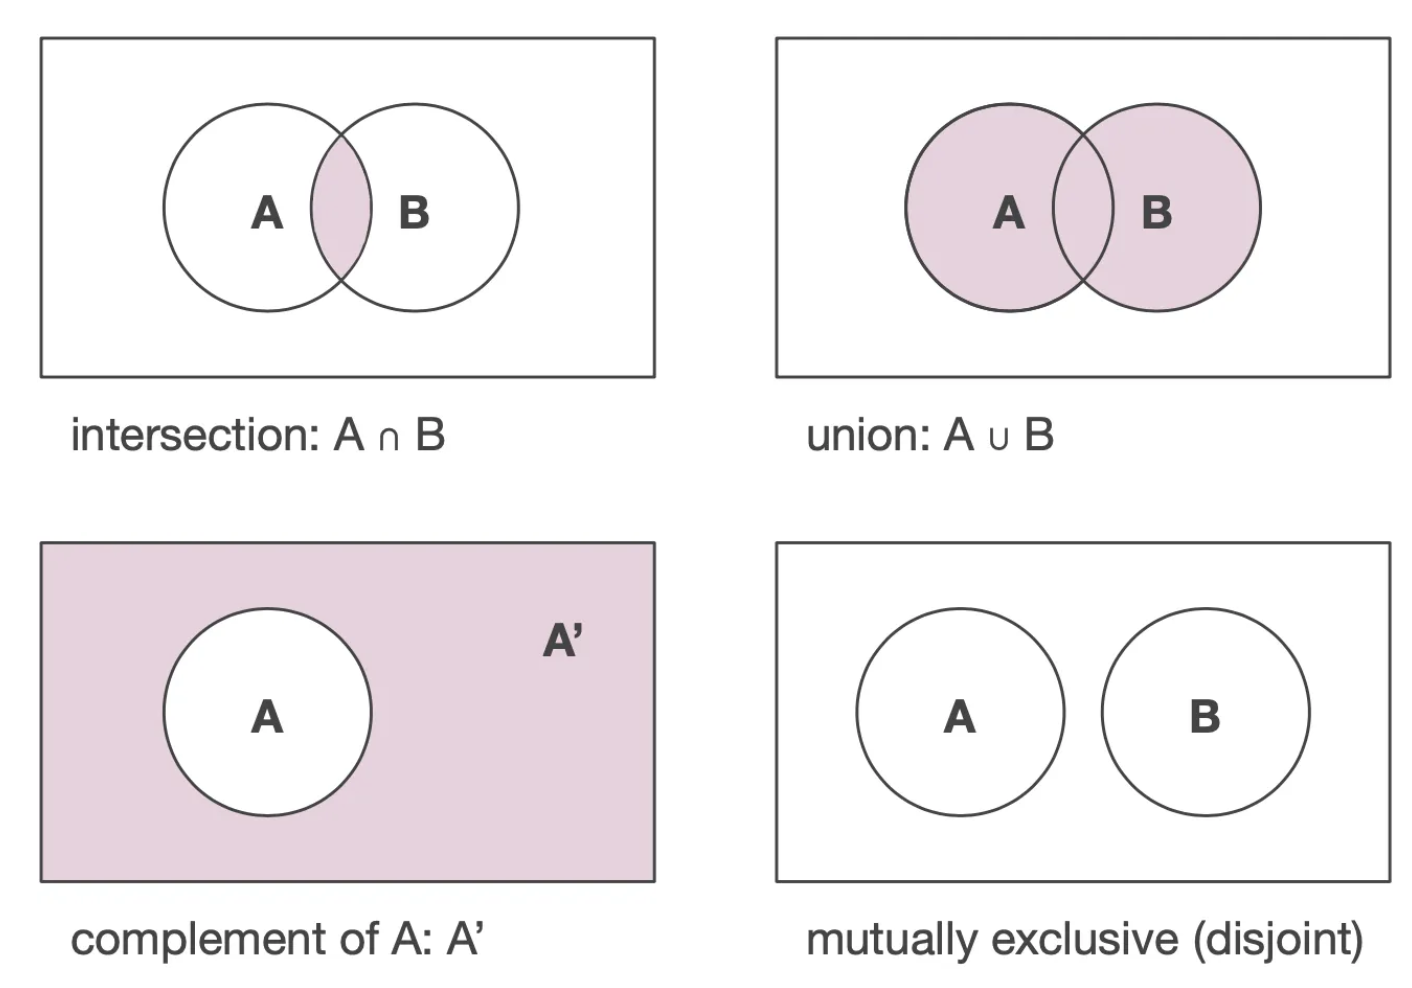
\includegraphics[scale=0.2]{img/sets.png}
\end{figure}

% \begin{itemize}
%     \item Intersection (AND): $A \cap B = \{2, 4, 6\} \cap \{4, 5, 6\} = \{4, 6\}$
%     \item Union (OR): $A \cup B = \{2, 4, 6\} \cup \{4, 5, 6\} = \{2, 4, 5, 6\}$
%     \item Complement (opposite): $A^C = \{2, 4, 6\}^C = \{1, 3, 5\}$
%     \item Mutually exclusive: $A$ and $A^C$ are mutually exclusive
% \end{itemize}

\begin{table}
\begin{tabular}{lrll}
Intersection &$A \cap B$&=$\{2, 4, 6\} \cap \{4, 5, 6\}$ &$=\{4, 6\}$ \\
Union &$A \cup B$&=$\{2, 4, 6\} \cup \{4, 5, 6\}$ &$=\{2, 4, 5, 6\}$ \\
Complement &$A^C$&=$\{2, 4, 6\}^C$ &$=\{1, 3, 5\}$ 
\end{tabular}
\end{table}
Question: are $A$ and $C$ mutually exclusive?

\end{frame}


%%%%%%%%%%%%%%%%%%%%%%%%%%%%%%%%%%%%%%%%%%%%%%%%%%%%%%%%%%%%%%%%%%%%%%%%%%%%%%%%
\begin{frame}{Probability Rules}

Several helpful rules follow from the aforementioned axioms.

\vspace{2ex}
\textbf{1. Complement Rule}: For any event A in the possible outcomes, the probabililty of A not happening (sometimes called the complement of $A$, or $A^C$) is:
\begin{equation*}
    \PP (\text{NOT } A) = \PP (A^C) = 1 - \PP(A)
\end{equation*}

\pause
\vspace{1ex}
\emph{Example: } You roll a die. The probability you roll a 2 is $\frac{1}{6}$:
\begin{equation*}
    \PP (\text{Roll a } 2) = \frac{1}{6}
\end{equation*}
What is the probability you roll either a 2, 3, 4, 5, or 6?

\pause
\emph{Answer: } Rolling a 2 is an event. The complement of this event is rolling a 2, 3, 4, 5, or 6:
\begin{align*}
    \PP (\{2, 3, 4, 5, 6\}) =& 1 - \PP (\{2\}) \\
    =& 1 - \frac{1}{6} \\
    =&\frac{5}{6}
\end{align*}

\vspace{1ex}
Practice: HW Question 1



\end{frame}


%%%%%%%%%%%%%%%%%%%%%%%%%%%%%%%%%%%%%%%%%%%%%%%%%%%%%%%%%%%%%%%%%%%%%%%%%%%%%%%%
\begin{frame}{Probability Rules (cont.)}


\textbf{2. Union of events}: For any events $A$ and $B$ (note: I'm not saying anything about these events being mutually exclusive): 
\begin{align*}
    \PP (A \text{ OR } B) = \PP (A \cup B) =& \PP (A) + \PP (B) - \PP (A \text{ AND } B) \\
    =& \PP (A) + \PP (B) - \PP (A \cap B)
\end{align*}

\pause
% \vspace{2ex}
\emph{Example}: When rolling a fair die, what is the probability of rolling an even number, or a number greater than or equal to 4?

% \vspace{2ex}
\emph{Answer}:
Define events $A$ and $B$ as:
\begin{equation*}
    A = \{\text{Roll an even number}\} = \{2, 4, 6\} \quad\quad
    B = \{\text{Roll } \geq 4\} = \{4, 5, 6\}
\end{equation*}
% Using the formula above:
% % \begin{align*}
% %     \PP (A) &= \PP (\{2, 4, 6\}) = \frac{1}{2} \\
% %     \PP (B) &= \PP (\{4, 5, 6\}) = \frac{1}{2} \\
% %     \PP (A \cap B) &= \PP (\{2, 4, 6\} \cap \{4, 5, 6\}) = \PP (\{4, 6\}) = \frac{1}{3} \\
% % \end{align*}
\vspace{2ex}
Finish on board. Practice: HW Question 2

\end{frame}

%%%%%%%%%%%%%%%%%%%%%%%%%%%%%%%%%%%%%%%%%%%%%%%%%%%%%%%%%%%%%%%%%%%%%%%%%%%%%%%%
\begin{frame}{Probability Rules (cont.)}

\textbf{3. Marginalization}

You can write the probability of any event $A$ in terms of $A \cap B$ and $A \cap B^C$. This is because $B$ and $B^C$ \textbf{partition} the universe of possible outcomes. Example:
\begin{align*}
    A &=\text{Rolling an even number} &&= \{2, 4, 6\} \\
    B &=\text{Rolling a number} \geq 4 &&= \{4, 5, 6\} \\
    B^C \onslide<2->{&&&= \{1, 2, 3\}}
\end{align*}
\onslide<3->
\begin{align*}
    \PP (A) &= \PP (A \cap B) + \PP (A \cap B^C) \\
    &= \PP (\{4, 6\}) + \PP (\{2\}) \\
    \onslide<4->{&= \frac{1}{3} + \frac{1}{6}}\onslide<5->{ = \frac{1}{2}}
\end{align*}
\onslide<6->
More generally, you can write $\PP (A)$ in terms of any sets $B_1, B_2, \dots, B_n$ that partition the universe of possible outcomes:
\begin{equation*}
    \PP (A) = \sum_{i=1}^n \PP (A \cap B_i) = \PP (A \cap B_1) + \PP (A \cap B_2) + \dots + \PP (A \cap B_n) 
\end{equation*}

\end{frame}

%%%%%%%%%%%%%%%%%%%%%%%%%%%%%%%%%%%%%%%%%%%%%%%%%%%%%%%%%%%%%%%%%%%%%%%%%%%%%%%%
\begin{frame}{Summary of probability rules (so far)}

\textbf{1. Complement Rule}: For any event A in the possible outcomes, the probability of A not happening (sometimes called the complement of $A$, or $A^C$) is:
\begin{equation*}
    \PP (\text{NOT } A) = \PP (A^C) = 1 - \PP(A)
\end{equation*}

\textbf{2. Union of events}: For any events $A$ and $B$ (note: I'm not saying anything about these events being mutually exclusive): 
\begin{align*}
    \PP (A \text{ OR } B) = \PP (A \cup B) =& \PP (A) + \PP (B) - \PP (A \text{ AND } B) \\
    =& \PP (A) + \PP (B) - \PP (A \cap B)
\end{align*}

\textbf{3. Marginalization}: For any sets $B_1, B_2, \dots, B_n$ that partition the universe of possible outcomes, $\PP (A)$ can be written as:
\begin{equation*}
    \PP (A) = \sum_{i=1}^n \PP (A \cap B_i) = \PP (A \cap B_1) + \PP (A \cap B_2) + \dots + \PP (A \cap B_n) 
\end{equation*}
\end{frame}


%%%%%%%%%%%%%%%%%%%%%%%%%%%%%%%%%%%%%%%%%%%%%%%%%%%%%%%%%%%%%%%%%%%%%%%%%%%%%%%%
\section{Random variables}
\miniframesoff
\begin{frame}
    \tableofcontents[currentsection]
\end{frame}
\miniframeson
%%%%%%%%%%%%%%%%%%%%%%%%%%%%%%%%%%%%%%%%%%%%%%%%%%%%%%%%%%%%%%%%%%%%%%%%%%%%%%%



%%%%%%%%%%%%%%%%%%%%%%%%%%%%%%%%%%%%%%%%%%%%%%%%%%%%%%%%%%%%%%%%%%%%%%%%%%%%%%%%
\begin{frame}{Random variables}

Random variables are probabilistic events mapped to real numbers. 
\begin{itemize}
    \item We need to map to real numbers to do any math!
\end{itemize}

% \vspace{2ex}
\onslide<2->
Example: Suppose we flip two coins and count the number of heads:
\begin{table}
\begin{tabular}{llc}
Flip 1 &Flip 2  &Final count ($X$) \\
\hline
Heads   &Heads  &2 \\
Heads   &Tails  &1 \\
Tails   &Heads  &1 \\
Tails   &Tails  &0 
\end{tabular}
\end{table}

\onslide<3->
We can define our random variable $X$ over it's possible outcomes, $\{0, 1, 2\}$:
\begin{table}
\begin{tabular}{cl}
$X$ &$\PP (X = x)$ \\
\hline
0 & $\PP (X = 0) = \frac{1}{4}$\\
1 &$\PP (X = 1) = \frac{1}{2}$\\
2 &$\PP (X = 2) = \frac{1}{4}$\\
\end{tabular}
\end{table}



% $\PP\left( \frac{1}{2} \right)$ 
% $\PP\left( \frac{1}{2} \right)$

\end{frame}

%%%%%%%%%%%%%%%%%%%%%%%%%%%%%%%%%%%%%%%%%%%%%%%%%%%%%%%%%%%%%%%%%%%%%%%%%%%%%%%%
\begin{frame}{Discrete probability mass function (PMF)}
We can describe the probability of $X$ using the function $p_X(x)$, its \textbf{probability mass function}, \textbf{PMF} (sometimes called the \textbf{discrete probability density function}, or \textbf{PDF}).
\begin{equation*}
    p_X(x) = \begin{cases}
    \frac{1}{4} &\text{if } x = 0 \\
    \frac{1}{2} &\text{if }x=1 \\
    \frac{1}{4} &\text{if }x=2
    \end{cases}
\end{equation*}

The PMF can be described graphically: 
\begin{figure}
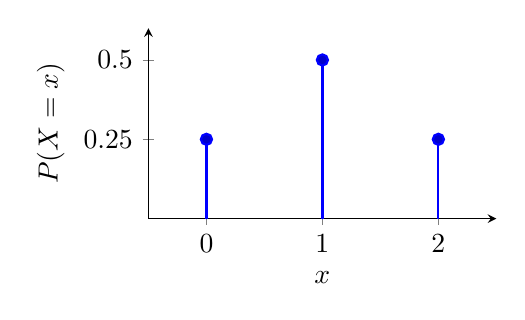
\begin{tikzpicture}
  \begin{axis}[
    ymin=0, ymax=0.6,
    xmin=-0.5, xmax=2.5,
    xtick={0,1,2},
    ytick={0.25,0.5},
    axis lines=left,
    width=6cm,
    height=4cm,
    xlabel={$x$},
    ylabel={$P(X = x)$},
    samples=3,
    domain=0:2,
    % enlargelimits=0.1,
    every axis plot/.append style={ultra thick}
  ]
  
  % Vertical lines
  \addplot+[ycomb, mark=*, blue, thick] coordinates {
    (0, 0.25)
    (1, 0.5)
    (2, 0.25)
  };

  \end{axis}
\end{tikzpicture}
\end{figure}


\end{frame}


%%%%%%%%%%%%%%%%%%%%%%%%%%%%%%%%%%%%%%%%%%%%%%%%%%%%%%%%%%%%%%%%%%%%%%%%%%%%%%%%
\begin{frame}{Continuous vs. Discrete random variable}

The examples on the previous slide are DISCRETE random variables (i.e. they take on a finite number of values)

\vspace{2ex}
Random variables can also be continuous. Examples:
\begin{itemize}
    \item Height of a random person selected in the population
    \item The time it takes you to commute to Hunter
    \item The temperature in Central Park at 10AM
\end{itemize}

\vspace{2ex}
These random variables take on an uncountably infinite number of values (even within a small interval)
\begin{itemize}
    \item Because each point in an interval is infinitely small, non-zero probabilities for continuous random variables are generally expressed as ranges
\begin{align*}
    \PP (45 \text{ minutes} < \text{My commute} \leq 60 \text{ minutes})
\end{align*}
\end{itemize}
Similar to how we used the \textbf{PMF} to describe probabilities for discrete random variables, we can describe probabilities for continuous random variables using the \textbf{probability density function} (\textbf{PDF}).

\end{frame}

%%%%%%%%%%%%%%%%%%%%%%%%%%%%%%%%%%%%%%%%%%%%%%%%%%%%%%%%%%%%%%%%%%%%%%%%%%%%%%%%
\begin{frame}{Probability Density Function}

Suppose $X$ follows a normal distribution with mean $\mu$ and standard deviation $\sigma$. The PDF for $X$, $f_X$, looks like:
\begin{figure}[width=0.25\textwidth]
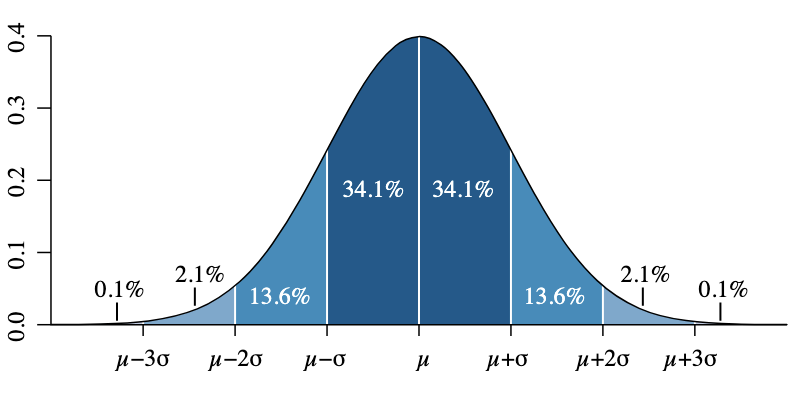
\includegraphics[scale=0.5]{img/normal_distribution.png}
\end{figure}
Then the probability that $X$ follows within one standard devation of the mean can be calculated by the area under the curve:
\begin{equation*}
    \PP (\mu - \sigma \leq X \leq \mu + \sigma) = 0.682
\end{equation*}


\end{frame}

%%%%%%%%%%%%%%%%%%%%%%%%%%%%%%%%%%%%%%%%%%%%%%%%%%%%%%%%%%%%%%%%%%%%%%%%%%%%%%%%
\begin{frame}{Continuous PDF}

In general, for some continuous random variable $X$ with density $f_X$, the probability is given by the area under the curve:
\begin{equation*}
    \PP (a \leq x \leq b) = \int_a^b f_X(x) dx
\end{equation*}

We won't make you do calculus in this class!  We'll focus on discrete random variables, but be aware that the infrastructure exists to deal with continuous random variables.

\end{frame}

%%%%%%%%%%%%%%%%%%%%%%%%%%%%%%%%%%%%%%%%%%%%%%%%%%%%%%%%%%%%%%%%%%%%%%%%%%%%%%%%
\begin{frame}{Cumulative distribution function (CDF)}

A cumulative distribution function is simply the probability that a random variable $X$ is less than or equal to some value:
\begin{equation*}
    F_X (x) = \PP (X \leq x)
\end{equation*}

\end{frame}


%%%%%%%%%%%%%%%%%%%%%%%%%%%%%%%%%%%%%%%%%%%%%%%%%%%%%%%%%%%%%%%%%%%%%%%%%%%%%%%%
\begin{frame}{Discrete CDF example}



\begin{figure}
\centering
\begin{subfigure}{0.4\textwidth}
\caption{Probability Mass Function}
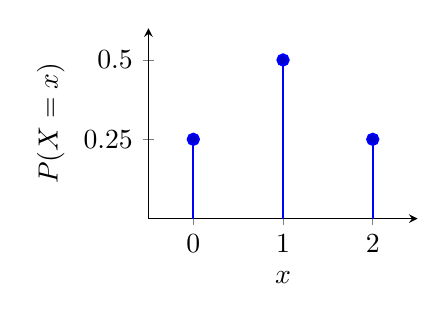
\begin{tikzpicture}
  \begin{axis}[
    ymin=0, ymax=0.6,
    xmin=-0.5, xmax=2.5,
    xtick={0,1,2},
    ytick={0.25,0.5},
    axis lines=left,
    width=5cm,
    height=4cm,
    xlabel={$x$},
    ylabel={$P(X = x)$},
    samples=3,
    domain=0:2,
    % enlargelimits=0.1,
    every axis plot/.append style={ultra thick}
  ]
  
  % Vertical lines
  \addplot+[ycomb, mark=*, blue, thick] coordinates {
    (0, 0.25)
    (1, 0.5)
    (2, 0.25)
  };

  \end{axis}
\end{tikzpicture}
\end{subfigure}

\hspace{3ex}

\begin{subfigure}{0.4\textwidth}
\caption{Cumulative Distribution Function}
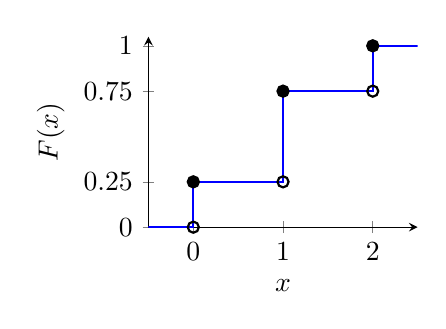
\begin{tikzpicture}
  \begin{axis}[
    axis x line=bottom,
    axis y line=left,
    xmin=-0.5, xmax=2.5,
    ymin=0, ymax=1.05,
    xtick={0,1,2},
    ytick={0,0.25,0.75,1},
    width=5cm,
    height=4cm,
    xlabel={$x$},
    ylabel={$F(x)$},
  ]
    % Step plot of CDF
    \addplot+[const plot, no marks, thick] coordinates {
      (-0.5, 0)
      (0, 0.25)
      (1, 0.75)
      (2, 1)
      (2.5, 1)
    };
    % Closed dots at jumps
    \addplot[only marks, mark=*, thick] coordinates {
      (0, 0.25)
      (1, 0.75)
      (2, 1)
    };
    % Open dots at left-hand limits (just before each jump)
    \addplot[only marks, mark=o, thick] coordinates {
      (0, 0)
      (1, 0.25)
      (2, 0.75)
    };
  \end{axis}
\end{tikzpicture}
\end{subfigure}
\end{figure}

\end{frame}

%%%%%%%%%%%%%%%%%%%%%%%%%%%%%%%%%%%%%%%%%%%%%%%%%%%%%%%%%%%%%%%%%%%%%%%%%%%%%%%%
\begin{frame}{Continuous CDF}

\begin{figure}
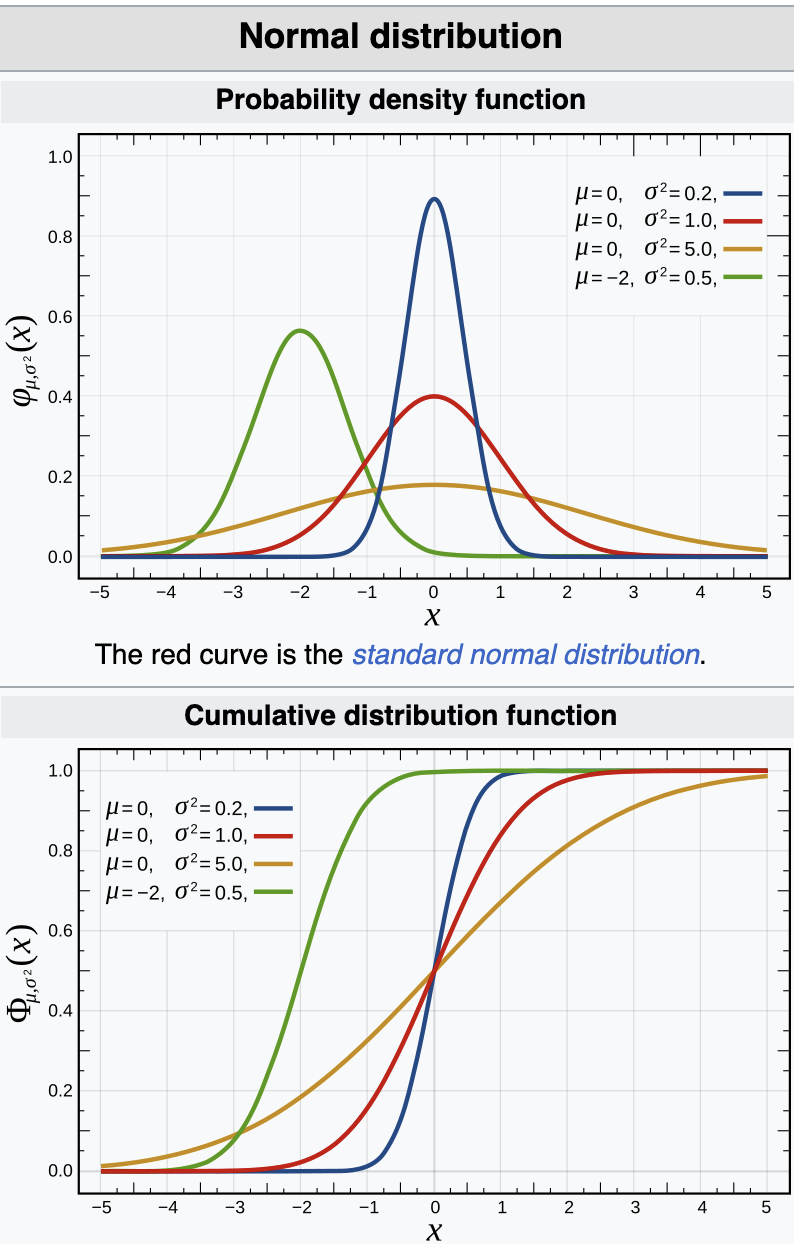
\includegraphics[scale=0.35]{img/normal_cdf.png}
\end{figure}

\end{frame}
%%%%%%%%%%%%%%%%%%%%%%%%%%%%%%%%%%%%%%%%%%%%%%%%%%%%%%%%%%%%%%%%%%%%%%%%%%%%%%%%

%%%%%%%%%%%%%%%%%%%%%%%%%%%%%%%%%%%%%%%%%%%%%%%%%%%%%%%%%%%%%%%%%%%%%%%%%%%%%%%%
\section{Independence}
\miniframesoff
\begin{frame}
    \tableofcontents[currentsection]
\end{frame}
\miniframeson
%%%%%%%%%%%%%%%%%%%%%%%%%%%%%%%%%%%%%%%%%%%%%%%%%%%%%%%%%%%%%%%%%%%%%%%%%%%%%%%


%%%%%%%%%%%%%%%%%%%%%%%%%%%%%%%%%%%%%%%%%%%%%%%%%%%%%%%%%%%%%%%%%%%%%%%%%%%%%%%%
\begin{frame}{Independence}

Two events are \textbf{independent} if the occurrence of $A$ does not impact the occurrence of $B$, and vice versa.

\vspace{3ex}
Very powerful concept. Recall our discussion last class about randomization:
\begin{itemize}
    \item We introduced the potential outcomes model, where $Y_0$ and $Y_1$ are the potential outcomes of $Y$
    \item If the treatment $D$ is independent of potential outcomes $(Y_0, Y_1)$, we write:
    \begin{equation*}
        Y_0, Y_1 \perp D
    \end{equation*}
    \item Treatment $D$ is randomly assigned if $D$ is independent of the potential outcomes
    \begin{itemize}
        \item[$\implies$] Randomization makes treatment and control groups comparable
        \item[$\implies$] Selection bias is zero
        \item[$\implies$] The average of observed differences in outcomes equals the average treatment effect
    \end{itemize}
\end{itemize}

\vspace{3ex}
To rigorously define independence, it helps to first define conditional probability. 

\end{frame}

%%%%%%%%%%%%%%%%%%%%%%%%%%%%%%%%%%%%%%%%%%%%%%%%%%%%%%%%%%%%%%%%%%%%%%%%%%%%%%%%
\begin{frame}{Conditional probability}

For two events $A$, and $B$, the conditional probability of $A$ given $B$, $\PP (A \vert B)$, is the probability of $A$ if $B$ is known. 
This is defined as:
\begin{equation*}
\PP (A \vert B) = \frac{\PP (A \text{ AND } B)}{\PP (B)} =  \frac{\PP (A \cap B)}{\PP (B)} = \frac{\PP (A, B)}{\PP (B)}
\end{equation*}

\vspace{2ex}
% Example: Suppose you are selecting a card from a standard deck of 52 cards. What is the probability that the card is even, given that the card is red?

% \begin{align*}
%     \PP(\text{Red}) &= \frac{26}{52} \\
%     \PP(\text{Even AND Red}) &= \frac{10}{52} \\
%     \PP(\text{Even} \vert \text{Red}) &= \frac{10/52}{26/52} = \frac{10}{26} = \frac{5}{13}
% \end{align*}

Example: Suppose you are selecting a card from a standard deck of 52 cards. What is the probability that the card is a heart, given that the card is red?
\begin{align*}
    \PP(\text{Red}) &= \frac{26}{52} \\
    \PP(\text{Heart AND Red}) &= \frac{13}{52} \\
    \PP(\text{Heart} \vert \text{Red}) &= \frac{13/52}{26/52} = \frac{1}{2} 
\end{align*}
Example: Suppose you have a standard deck of 52 cards. What is the probability that a card is black, given that it's a club? 


\end{frame}

%%%%%%%%%%%%%%%%%%%%%%%%%%%%%%%%%%%%%%%%%%%%%%%%%%%%%%%%%%%%%%%%%%%%%%%%%%%%%%%%
\begin{frame}{Conditional probability and independence}
\begin{enumerate}
    \item Conditional probability definition:
\begin{equation*}
\alert<3>{\PP (A \vert B)} = \alert<3>{\frac{\PP (A, B)}{\PP (B)}}   
\end{equation*}
\item Two events are independent if the occurrence of A does not impact the occurrence of B, and vice versa.
\end{enumerate}

\onslide<2->
\vspace{3ex}
Intuitively, it follows that if $A$ and $B$ are independent, then the probability of $A$ is unchanged if you know $B$. This implies:
\begin{equation*}
    \alert<4>{\PP (A \vert B) = \PP(A)}
\end{equation*}

\onslide<3->
Using the definition of conditional probability:
\begin{align*}
    \frac{\PP (A, B)}{\PP (B)} =& \PP (A \vert B) \\
    \onslide<4->{\implies \frac{\PP (A, B)}{\alert<5>{\PP (B)}} =&\alert<4>{\PP (A)}\\}
    \onslide<5->{\implies \PP (A, B) =& \PP(A) \alert<5>{\PP(B)}}
\end{align*}

\onslide<6->
Formally: Events are \textbf{independent} if and only if their joint probability equals the product of their probabilities

\end{frame}

%%%%%%%%%%%%%%%%%%%%%%%%%%%%%%%%%%%%%%%%%%%%%%%%%%%%%%%%%%%%%%%%%%%%%%%%%%%%%%%%
\begin{frame}{Independence Example}

Consider rolling a die twice
\begin{itemize}
    \item $X$: the outcome of roll 1
    \item $Y$: the outcome of roll 2
\end{itemize}
Intuitively, it makes sense that the occurrence of $X$ does not impact the occurrence of $Y$, and vice versa.
\begin{itemize}
    \item $X$ and $Y$ are independent
\end{itemize}
What is the probability that the second roll equals 2, given that you know the first roll equals 1?
\begin{align*}
    \PP (Y = 2 \vert X = 1) &= \PP (Y = 2)
\end{align*}
In general, because $X$ and $Y$ are independent:
\begin{equation*}
    \PP (Y \vert X) = \PP (Y)
\end{equation*}

\end{frame}

%%%%%%%%%%%%%%%%%%%%%%%%%%%%%%%%%%%%%%%%%%%%%%%%%%%%%%%%%%%%%%%%%%%%%%%%%%%%%%%%
\begin{frame}{Independence examples (cont.)}

Given events:
\begin{itemize}
    \item Month $M \in \{\text{Jan}, \text{Feb}, \dots, \text{Dec}\}$
    \item Weather $W \in \{\text{sunny}, \text{rainy}\}$
    \onslide<3->{\alert<3>{\item Day of the week $D \in \{\text{Mon.}, \dots, \text{Sun}\}$}}
\end{itemize}
Suppose:
\begin{align*}
    \PP (W = \text{sunny}) &= 0.9 \\
    \PP (W = \text{sunny} \vert M = \text{Aug.}) &= 0.93 \\
    \PP (W = \text{sunny} \vert M = \text{Jan.}) &= 0.83 \\
    \onslide<3->{\PP (W = \text{sunny} \vert D = \text{Tues.}) &= 0.9 \\}
    \onslide<3->{\PP (W = \text{sunny} \vert D = \text{Fri.}) &= 0.9}
\end{align*}
Are month and weather independent? \onslide<2->{\alert<2>{No}, month and weather are \alert<2>{dependent}:
\begin{equation*}
    \PP (W \vert M) \neq \PP (W)
 \end{equation*} 
 }
 \onslide<3->{Are weather and day of the week independent?} \onslide<4->{\alert<4>{Yes}:
 \begin{equation}
     \PP (W \vert D) = \PP (W)
 \end{equation}
}
\end{frame}

%%%%%%%%%%%%%%%%%%%%%%%%%%%%%%%%%%%%%%%%%%%%%%%%%%%%%%%%%%%%%%%%%%%%%%%%%%%%%%%%
\section{Conditional Probability Rules}
\miniframesoff
\begin{frame}
    \tableofcontents[currentsection]
\end{frame}
\miniframeson
%%%%%%%%%%

%%%%%%%%%%%%%%%%%%%%%%%%%%%%%%%%%%%%%%%%%%%%%%%%%%%%%%%%%%%%%%%%%%%%%%%%%%%%%%%%
\begin{frame}{Recall laws of probability}

\textbf{1. Complement Rule}: For any event A in the possible outcomes, the probability of A not happening (sometimes called the complement of $A$, or $A^C$) is:
\begin{equation*}
    \PP (\text{NOT } A) = \PP (A^C) = 1 - \PP(A)
\end{equation*}

\textbf{2. Union of events}: For any events $A$ and $B$ (note: I'm not saying anything about these events being mutually exclusive): 
\begin{align*}
    \PP (A \text{ OR } B) = \PP (A \cup B) =& \PP (A) + \PP (B) - \PP (A \text{ AND } B) \\
    =& \PP (A) + \PP (B) - \PP (A \cap B)
\end{align*}

\textbf{3. Marginalization}: For any sets $B_1, B_2, \dots, B_n$ that partition the universe of possible outcomes, $\PP (A)$ can be written as:
\begin{equation*}
    \PP (A) = \sum_{i=1}^n \PP (A \cap B_i) = \PP (A \cap B_1) + \PP (A \cap B_2) + \dots + \PP (A \cap B_n) 
\end{equation*}

\vspace{3ex}
Let's consider how some of these laws apply to conditional probability!

\end{frame}

%%%%%%%%%%%%%%%%%%%%%%%%%%%%%%%%%%%%%%%%%%%%%%%%%%%%%%%%%%%%%%%%%%%%%%%%%%%%%%%%
\begin{frame}{Conditional probability}

In general, conditional probabilities are still probabilities, so the rules on the previous page still apply. For example:


\vspace{3ex}
\textbf{Complement Rule}: For any event A in the possible outcomes, the probability of A not happening (sometimes called the complement of $A$, or $A^C$) is:
\begin{equation*}
    \PP (\text{NOT } A) = \PP (A^C) = 1 - \PP(A)
\end{equation*}
This law applies under conditional probability:
\begin{equation*}
    \PP (A^C \vert B) = 1 - \PP(A \vert B)
\end{equation*}

\pause
\vspace{3ex}
Example: Suppose we have a drug test for marijuana. We know it correctly identifies non-users as non-users 80\% of the time:
\begin{equation*}
    \PP (\text{Test negative} \vert \text{Non-user}) = 0.8
\end{equation*}
What is the probability that the drug test incorrectly identifies a non-user as a user? (This is called the \textbf{False Positive Rate}).
\pause
\begin{equation*}
    \PP (\text{Test positive} \vert \text{Non-user}) = 1 - 0.8 = 0.2    
\end{equation*}

\end{frame}



%%%%%%%%%%%%%%%%%%%%%%%%%%%%%%%%%%%%%%%%%%%%%%%%%%%%%%%%%%%%%%%%%%%%%%%%%%%%%%%%
\begin{frame}{Laws of Probability - Law of Total Probability}

Now we have our definition of conditional probability:
\begin{equation*}
\PP (A \vert B) = \frac{\PP (A \cap B)}{\PP (B)} \implies \PP (A \cap B) = \PP (A \vert B) \PP (B)
\end{equation*}

Recall \textbf{marginalization}: For any sets $B_1, B_2, \dots, B_n$ that partition the universe of possible outcomes, $\PP (A)$ can be written as:
\begin{equation*}
    \PP (A) = \sum_{i=1}^n \PP (A \cap B_i) = \PP (A \cap B_1) + \PP (A \cap B_2) + \dots + \PP (A \cap B_n) 
\end{equation*}

Note that we can re-write this rule using the definition of conditional probability:
\begin{equation*}
    \PP (A) = \sum_{i=1}^n \PP (A \vert B_i) \PP (B_i)
\end{equation*}
This is the \textbf{Law of Total Probability}.


\end{frame}

%%%%%%%%%%%%%%%%%%%%%%%%%%%%%%%%%%%%%%%%%%%%%%%%%%%%%%%%%%%%%%%%%%%%%%%%%%%%%%%%
\begin{frame}{Law of Total Probability Example}

Suppose we have a drug test for marijuana.
\begin{equation*}
     M = \begin{cases} 1 &\text{ if person uses marijuana} \\
     0 &\text{ if person does not use marijuana} \end{cases}
     \quad\quad
     P = \begin{cases} 1 &\text{ if test result is positive} \\
     0 &\text{ if test result is negative} \end{cases}
 \end{equation*} This test has a 90\% \href{https://en.wikipedia.org/wiki/Sensitivity_and_specificity}{true positive rate}, meaning that if someone does use marijuana, the test will accurately predict them as a user 90\% of the time.
\begin{equation*}
    \PP (\text{Positive} \vert \text{User}) = \PP (P = 1 \vert M =1 ) = 0.9
\end{equation*}
The test also has a true negative rate equal to 80\%. This means that someone who does not use marijuana is receives a negative test result 80\% of the time:
\begin{align*}
    \PP (\text{Negative} \vert \text{Non-user}) =& \PP (P = 0 \vert M = 0) = 0.8
\end{align*}
Finally, suppose the prevalence of marijuana usage in the population is 5\%. This means 5\% of people use marijuana:
\begin{equation*}
    \PP (\text{User}) = \PP (M = 1) = 0.05
\end{equation*}
For a randomly selected person, what is the probability the test is positive, $\PP (P = 1)$?

\end{frame}

%%%%%%%%%%%%%%%%%%%%%%%%%%%%%%%%%%%%%%%%%%%%%%%%%%%%%%%%%%%%%%%%%%%%%%%%%%%%%%%%
\begin{frame}{Law of Total Probability Example}

Using the law of total probability, we can re-write $\PP (P)$ as:
\begin{align*}
    \PP (P = 1) &= \PP (P = 1 \vert M = 0 ) \PP (M = 0) + \PP (P = 1 \vert M = 1) \PP (M=1)
\end{align*}
Using the true positive rate and the prevalence, we can re-write this as:
\begin{align*}
    \PP (P = 1) &= \PP (P = 1 \vert M = 0 ) \PP (M = 0) + 0.9 \cdot 0.05
\end{align*}
By the \textbf{complement rule}, we know:
\begin{align*}
    \PP (M = 0) &= 1 - \PP (M = 1) = 1 - 0.05 = 0.95
\end{align*}
The complement rule also applies to conditional probability, so we know the \textbf{False positive rate}:
\begin{align*}
    \PP (P = 1 \vert M = 0 ) &= 1 - \PP (P = 0 \vert M = 0) = 1 - 0.8 = 0.2
\end{align*}
Meaning:
\begin{align*}
    \PP (P = 1) &= 0.2 \cdot 0.95 + 0.9 \cdot 0.05 \\
    &= 0.19 + 0.045 \\
    &= 0.235
\end{align*}
Therefore, the probability a randomly selected person tests positive is 23.5\%

\end{frame}


%%%%%%%%%%%%%%%%%%%%%%%%%%%%%%%%%%%%%%%%%%%%%%%%%%%%%%%%%%%%%%%%%%%%%%%%%%%%%%%%
\begin{frame}{Laws of Probability - Bayes Rules}

Definition of conditional probability for events $A$ and $B$:
\begin{equation*}
    \PP (A \vert B) = \frac{\PP (A, B)}{\PP (B)}
\end{equation*}
We can use the definition of conditional probability to define joint probabilities in an intuitive way. Note:
\begin{align*}
    \PP(A \vert B) \PP(B) &= \PP (A, B) \\
    \PP(B \vert A) \PP(A) &= \PP (A, B) \\
\end{align*}
Together, these equations imply \textbf{Bayes' Rule}:
\begin{equation*}
    \PP (A \vert B) = \frac{\PP (B \vert A) \PP(A)}{\PP(B)}
\end{equation*}
Bayes rule is powerful because it allows you to invert conditional probabilities!
\begin{itemize}
    \item $A$: Patient has a disease (cause)
    \item $B$: Patient tested positive for a disease (effect)
    \item Bayes rule allows one to find the probability of a cause given its effect
\end{itemize}
Easiest to see if we walk through an example



\end{frame}

%%%%%%%%%%%%%%%%%%%%%%%%%%%%%%%%%%%%%%%%%%%%%%%%%%%%%%%%%%%%%%%%%%%%%%%%%%%%%%%%
\begin{frame}{Bayes Rule example - drug testing}


Using the previous example, What is the probability that a randomly selected person who tests positive actually uses marijuana?

\vspace{3ex}
The \href{https://en.wikipedia.org/wiki/Positive_and_negative_predictive_values}{\textbf{positive predictive value (PPV)}} predicts the proportion of positive test results are true positives.
\begin{equation*}
    \PP (\text{User} \vert \text{Positive}) = \PP (M = 1 \vert P = 1)
\end{equation*}
Can use Bayes' Theorem to solve this:
\begin{align*}
    \PP (M = 1 \vert P = 1) &= \frac{\PP  (P = 1 \vert M = 1) \PP (M = 1)}{\PP (P = 1)} \\
    % &= \frac{\PP  (P = 1 \vert M = 1) \PP (M = 1)}{
        % \PP (P = 1 \vert M = 0 ) \PP (M = 0) + \PP (P = 1 \vert M = 1) \PP (M=1)} 
        % &= \PP ()
\end{align*}



\end{frame}

%%%%%%%%%%%%%%%%%%%%%%%%%%%%%%%%%%%%%%%%%%%%%%%%%%%%%%%%%%%%%%%%%%%%%%%%%%%%%%%%
\begin{frame}{Bayes Rule example - drug testing (cont.)}

True positive rate: 
\begin{equation*}
    \PP (\text{Positive} \vert \text{User}) = \PP (P = 1 \vert M =1 ) = 0.9
\end{equation*}
Prevalence:
\begin{equation*}
    \PP (\text{User}) = \PP (M = 1) = 0.05
\end{equation*}
Predicted positive:
\begin{align*}
    \PP (P = 1) &= 0.235
\end{align*}
Solving using Bayes Theorem:
\begin{align*}
    \PP (M = 1 \vert P = 1) &= \frac{\PP  (P = 1 \vert M = 1) \PP (M = 1)}{\PP (P = 1)} \\
    &= \frac{0.9 \cdot 0.05}{0.235} \\
    &= 0.19
        % &= \PP ()
\end{align*}
If someone tests positive, the probability that they are a cannabis user is only 19\%—because in this group, only 5\% of people are users, and most positives are false positives coming from the remaining 95\%. 

\end{frame}

%%%%%%%%%%%%%%%%%%%%%%%%%%%%%%%%%%%%%%%%%%%%%%%%%%%%%%%%%%%%%%%%%%%%%%%%%%%%%%%%
\begin{frame}{Bayes Rule example - drug testing (cont.)}

\begin{figure}
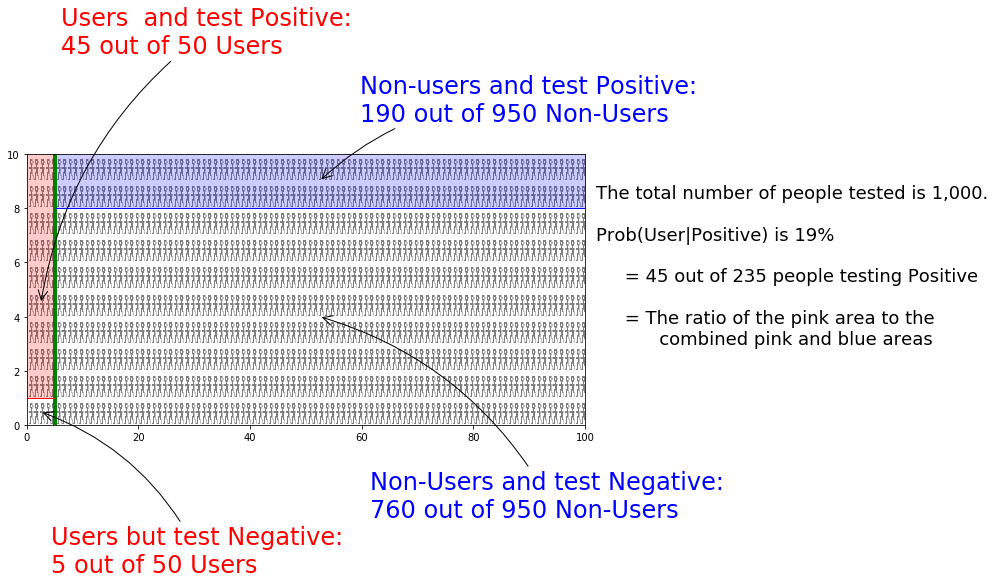
\includegraphics[scale=0.3]{img/bayes_rule.png}
\end{figure}

\end{frame}



%%%%%%%%%%%%%%%%%%%%%%%%%%%%%%%%%%%%%%%%%%%%%%%%%%%%%%%%%%%%%%%%%%%%%%%%%%%%%%%%
\section{Conditional Independence}
\miniframesoff
\begin{frame}
    \tableofcontents[currentsection]
\end{frame}
\miniframeson
%%%%%%%%%%



%%%%%%%%%%%%%%%%%%%%%%%%%%%%%%%%%%%%%%%%%%%%%%%%%%%%%%%%%%%%%%%%%%%%%%%%%%%%%%%%
\begin{frame}{Conditional Independence example}

Consider the binary variables:
\begin{itemize}
    \item $R \in \{0, 1\}$: Student $R$ aced the test
    \item $S \in \{0, 1\}$: Student $S$ aced the test
    \item $T \in \{0, 1\}$: The test is hard
\end{itemize}
    
\begin{figure}
\begin{tikzpicture}
\node [draw, circle] (T) {T};
\node [draw, circle, below right =of T] (S) {S};
\node [draw, circle, below left =of T] (R) {R};
\draw (T) edge[->] (R);
\draw (T) edge[->] (S);
\end{tikzpicture}
\end{figure}

Are $R$ and $S$ independent? Independence means, for example:
\begin{equation*}
    \PP (R = 1\vert S=1) = \PP (R = 1)
\end{equation*}
In words, if we know student $S$ aced the test, does that give us any information about whether student $R$ aced the test?

\pause
\begin{itemize}
    \item These variables are \textbf{marginally dependent (unconditionally dependent)}; the occurrence of one impacts the occurrence of the other
\end{itemize}

\end{frame}


%%%%%%%%%%%%%%%%%%%%%%%%%%%%%%%%%%%%%%%%%%%%%%%%%%%%%%%%%%%%%%%%%%%%%%%%%%%%%%%%
\begin{frame}{Conditional independence example (cont.)}

\begin{itemize}
    \item $R \in \{0, 1\}$: Student $R$ aced the test
    \item $S \in \{0, 1\}$: Student $S$ aced the test
    \item $T \in \{0, 1\}$: The test is hard
\end{itemize}

\begin{figure}
\begin{tikzpicture}
\node [draw, circle] (T) {T};
\node [draw, circle, below right =of T] (S) {S};
\node [draw, circle, below left =of T] (R) {R};
\draw (T) edge[->] (R);
\draw (T) edge[->] (S);
\end{tikzpicture}
\end{figure}

Are $R$ and $S$ independent, conditional on the difficulty of the test? Conditional independence means, for example:
\begin{equation*}
    \PP (R = 1\vert S=1, T=0) = \PP (R = 1 \vert T=0)
\end{equation*}
In words, if we know that the test was easy, does the additional information that student $S$ aced the test tell us anything about whether student $R$ aced the test?
\begin{itemize}
    \item If all the information you could glean from $S$ is subsumed in knowing the value of $T$, then $R$ and $S$ are independent conditional on $T$
\end{itemize}

\end{frame}

%%%%%%%%%%%%%%%%%%%%%%%%%%%%%%%%%%%%%%%%%%%%%%%%%%%%%%%%%%%%%%%%%%%%%%%%%%%%%%%%
\begin{frame}{Conditional Independence}


For any random variables $X$, $Y$, and $Z$, $X$ and $Y$ are \textbf{conditionally independent} given $Z$ if:
\begin{equation*}
    \PP (X = x \vert Y = y, Z = z) = \PP (X = x \vert Z = z)
\end{equation*}
In words, this means that learning $Y$ does not provide any additional information about $X$, once we learn $Z$. We'll often summarize conditional independence as:
\begin{equation*}
    X \perp Y \vert Z
\end{equation*}
\begin{itemize}
    \item Note this must hold for all values of $X$, $Y$, and $Z$ for conditional independence to hold
\end{itemize}

\end{frame}

%%%%%%%%%%%%%%%%%%%%%%%%%%%%%%%%%%%%%%%%%%%%%%%%%%%%%%%%%%%%%%%%%%%%%%%%%%%%%%%%
\begin{frame}{Causal Graphs}

\textbf{Simple graph 1 - Mediation}: $A \rightarrow C \rightarrow B$:
\begin{figure}
\begin{tikzpicture}
\node [draw, circle] (A) {A};
\node [draw, circle, right =of A] (C) {C};
\node [draw, circle, right =of C] (B) {B};
\draw (A) edge[->] (C);
\draw (C) edge[->] (B);
\end{tikzpicture}
\end{figure}
\begin{itemize}
    \item $A$ and $B$ are \textbf{marginally dependent}
    \item $A$ and $B$ are independent conditional on $C$: $A \perp B \vert C$
\end{itemize}

\textbf{Simple graph 2 - Mutual dependence}: $A \leftarrow C \rightarrow B$:
\begin{figure}
\begin{tikzpicture}
\node [draw, circle] (C) {C};
\node [draw, circle, below left =of C] (A) {A};
\node [draw, circle, below right =of C] (B) {B};
\draw (C) edge[->] (A);
\draw (C) edge[->] (B);
\end{tikzpicture}
\end{figure}
\begin{itemize}
    \item $A$ and $B$ are \textbf{marginally dependent} through mutual dependence on $C$
    \item $A$ and $B$ are independent conditional on $C$: $A \perp B \vert C$
\end{itemize}

\end{frame}

% %%%%%%%%%%%%%%%%%%%%%%%%%%%%%%%%%%%%%%%%%%%%%%%%%%%%%%%%%%%%%%%%%%%%%%%%%%%%%%%%
% \begin{frame}{Conditional independence example (cont.)}

% \begin{itemize}
%     \item $R \in \{0, 1\}$: Student $R$ aced the test
%     \item $S \in \{0, 1\}$: Student $S$ aced the test
%     \item $T \in \{0, 1\}$: The test is hard
% \end{itemize}

% \begin{figure}
% \begin{tikzpicture}
% \node [draw, circle] (T) {T};
% \node [draw, circle, below right =of T] (S) {S};
% \node [draw, circle, below left =of T] (R) {R};
% \draw (T) edge[->] (R);
% \draw (T) edge[->] (S);
% \end{tikzpicture}
% \end{figure}

% % Are $R$ and $S$ independent, conditional on the difficulty of the test? Conditional independence means, for example:
% % \begin{equation*}
% %     \PP (R = 1\vert S=1, T=0) = \PP (R = 1 \vert T=0)
% % \end{equation*}
% % In words, if we know that the test was easy, does the additional information that student $S$ aced the test tell us anything about whether student $R$ aced the test?
% % \begin{itemize}
% %     \item If all the information you could glean from $S$ is subsumed in knowing the value of $T$, then $R$ and $S$ are independent $conditional$ on $T$
% % \end{itemize}

% \end{frame}

%%%%%%%%%%%%%%%%%%%%%%%%%%%%%%%%%%%%%%%%%%%%%%%%%%%%%%%%%%%%%%%%%%%%%%%%%%%%%%%%
\begin{frame}{Conditional dependence}

Suppose College A requires students to have a high High School GPA or great musical talent in order to be admitted
\begin{itemize}
    \item $X \in \{0, 1\}$: A student has a high GPA
    \item $Y \in \{0, 1\}$: A student is musically talented
    \item $Z \in \{0, 1\}$: A student is admitted to College A
\end{itemize}
\begin{figure}
\begin{tikzpicture}
\node [draw, circle] (Z) {Z};
\node [draw, circle, above right =of Z] (Y) {Y};
\node [draw, circle, above left =of Z] (X) {X};
\draw (X) edge[->] (Z);
\draw (Y) edge[->] (Z);
\end{tikzpicture}
\end{figure}

Are $X$ and $Y$ independent of one another? Independence implies, for example, that knowing a student has a high GPA doesn't influence your probability that they are musically talented
    \begin{equation*}
    \PP (X =1 \vert Y=1) = \PP (X=1)
    \end{equation*}
 
\end{frame}

%%%%%%%%%%%%%%%%%%%%%%%%%%%%%%%%%%%%%%%%%%%%%%%%%%%%%%%%%%%%%%%%%%%%%%%%%%%%%%%%
\begin{frame}{Conditional dependence (cont.)}

\begin{itemize}
    \item $X \in \{0, 1\}$: A student has a high GPA
    \item $Y \in \{0, 1\}$: A student is musically talented
    \item $Z \in \{0, 1\}$: A student is admitted to College A
\end{itemize}
\begin{figure}
\begin{tikzpicture}
\node [draw, circle] (Z) {Z};
\node [draw, circle, above right =of T] (Y) {Y};
\node [draw, circle, above left =of T] (X) {X};
\draw (X) edge[->] (Z);
\draw (Y) edge[->] (Z);
\end{tikzpicture}
\end{figure}

\begin{itemize}
    \item Consider the probability a student has a high GPA, given that they were admitted to this college: $\PP (X = 1 \vert Z = 1)$
    \item Now consider the case where you know the student is musically talented AND was admitted to this college. You now have reason to think the musical talent is the cause of admission, not the high GPA. Is there reason to think:

    \begin{equation*}
    \PP (X =1 \vert Z=1) > \PP (X=1 \vert Y=1, Z=1)
    \end{equation*}

    \item \textbf{Conditional dependence} can happen when two causes have the same effect. You don't want to control on everything!
\end{itemize}

% \begin{frame}{}

% \begin{itemize}
%     \item $X \in \{0, 1\}$: There is an accident at an intersection
%     \item $Y \in \{0, 1\}$: There is a long red light at an intersection
%     \item $Z \in \{0, 1\}$: There is traffic at an intersection
% \end{itemize}
% \begin{figure}
% \begin{tikzpicture}
% \node [draw, circle] (Z) {Z};
% \node [draw, circle, above right =of T] (Y) {Y};
% \node [draw, circle, above left =of T] (X) {X};
% \draw (X) edge[->] (Z);
% \draw (Y) edge[->] (Z);
% \end{tikzpicture}
% \end{figure}

% \begin{itemize}
%     \item Consider the probability of an accident, given that there is traffic: $\PP (X = 1 \vert Z = 1)$
%     \item Now consider the case where know this intersection has a long traffic light, in addition to traffic. You now have reason to think the long light is the cause of the traffic, not a potential accident. Is there reason to think:

%     \begin{equation*}
%     \PP (X =1 \vert Z=1) > \PP (X=1 \vert Y=1, Z=1)
%     \end{equation*}

%     \item \textbf{Conditional dependence} can happen when two causes have the same effect. You don't want to control on everything!
% \end{itemize}




\end{frame}


%%%%%%%%%%%%%%%%%%%%%%%%%%%%%%%%%%%%%%%%%%%%%%%%%%%%%%%%%%%%%%%%%%%%%%%%%%%%%%%%
\begin{frame}{Causal Graphs (cont.)}


\textbf{Simple graph 3 - Mutual causation}: $A \rightarrow C \leftarrow B$:
\begin{figure}
\begin{tikzpicture}
\node [draw, circle] (C) {C};
\node [draw, circle, above left =of C] (A) {A};
\node [draw, circle, above right =of C] (B) {B};
\draw (A) edge[->] (C);
\draw (B) edge[->] (C);
\end{tikzpicture}
\end{figure}
\begin{itemize}
    \item If nothing is known about $C$, then knowing $A$ yields no additional information about $B$; 
    \item $A$ and $B$ are \textbf{marginally independent}
    \item Conditional on $C$, $A$ and $B$ are \textbf{dependent}
\end{itemize}

\end{frame}



% %%%%%%%%%%%%%%%%%%%%%%%%%%%%%%%%%%%%%%%%%%%%%%%%%%%%%%%%%%%%%%%%%%%%%%%%%%%%%%%%
% \section{Expectation}
% \miniframesoff
% \begin{frame}
%     \tableofcontents[currentsection]
% \end{frame}
% \miniframeson
% %%%%%%%%%%%%%%%%%%%%%%%%%%%%%%%%%%%%%%%%%%%%%%%%%%%%%%%%%%%%%%%%%%%%%%%%%%%%%%%


% %%%%%%%%%%%%%%%%%%%%%%%%%%%%%%%%%%%%%%%%%%%%%%%%%%%%%%%%%%%%%%%%%%%%%%%%%%%%%%%%
% \begin{frame}{}



% \end{frame}







\end{document}